\documentclass[lecture,12pt,]{pcms-l}
\input preamble.tex

% For faster processing, load Matlab syntax for listings
\definecolor{MyDarkGreen}{rgb}{0.0,0.4,0.0}
\lstloadlanguages{Matlab}%
\lstset{language=Matlab,
        frame=single,
        basicstyle=\small\ttfamily,
        keywordstyle=[1]\color{Blue}\bf,
        keywordstyle=[2]\color{Purple},
        keywordstyle=[3]\color{Blue}\underbar,
        identifierstyle=,
        commentstyle=\usefont{T1}{pcr}{m}{sl}\color{MyDarkGreen}\small,
        stringstyle=\color{Purple},
        showstringspaces=false,
        tabsize=5,
        % Put standard MATLAB functions not included in the default
        % language here
        morekeywords={xlim,ylim,var,alpha,factorial,poissrnd,normpdf,normcdf},
        % Put MATLAB function parameters here
        morekeywords=[2]{on, off, interp},
        % Put user defined functions here
        morekeywords=[3]{FindESS},
        morecomment=[l][\color{Blue}]{...},
        numbers=left,
        firstnumber=1,
        numberstyle=\tiny\color{Blue},
        stepnumber=0
        }

% Only the next five fields need to be edited.
\newcommand{\lecAuth}{R.A. de Callafon}
\newcommand{\scribe}{Thomas Denewiler}
\newcommand{\authEmail}{callafon@ucsd.edu}
\newcommand{\scribeEmail}{tdenewiler@gmail.com}
\newcommand{\course}{MAE 283: Parameter Estimation}
\newcommand{\lectureNum}{4}

\address{Department of Mechanical and Aerospace Engineering, University of California, San Diego}

% Adds a hyperlink to an email address.
\newcommand{\mailto}[2]{\href{mailto:#1}{#2}}

% These commands set the document properties for the PDF output. Needs the hyperref package.
\hypersetup
{
    colorlinks,
    linkcolor={black},
    citecolor={black},
    filecolor={black},
    urlcolor={black},
    pdfauthor={\scribe <\mailto{\scribeEmail}{\scribeEmail}>},
    pdfsubject={\course},
    pdftitle={Lecture \lectureNum},
    pdfkeywords={UC San Diego, Parameter Estimation, System Identification},
    pdfstartpage={1},
}

% Includes a figure
% The first parameter is the label, which is also the name of the figure
%   with or without the extension (e.g., .eps, .fig, .png, .gif, etc.)
%   IF NO EXTENSION IS GIVEN, LaTeX will look for the most appropriate one.
%   This means that if a DVI (or PS) is being produced, it will look for
%   an eps. If a PDF is being produced, it will look for nearly anything
%   else (gif, jpg, png, et cetera). Because of this, when I generate figures
%   I typically generate an eps and a png to allow me the most flexibility
%   when rendering my document.
% The second parameter is the width of the figure normalized to column width
%   (e.g. 0.5 for half a column, 0.75 for 75% of the column)
% The third parameter is the caption.
\newcommand{\scalefig}[3]{
  \begin{figure}[ht!]
    % Requires \usepackage{graphicx}
    \centering
	\fbox{
	    \includegraphics[width=#2\columnwidth]{#1}
	}
    %%% I think \captionwidth (see above) can go away as long as
    %%% \centering is above
    %\captionwidth{#2\columnwidth}%
    \caption{#3}
    \label{#1}
  \end{figure}}

% Includes a MATLAB script.
% The first parameter is the label, which also is the name of the script
%   without the .m.
% The second parameter is the optional caption.
\newcommand{\matlabscript}[2]
  {\begin{itemize}\item[]\lstinputlisting[caption=#2,label=#1]{#1.m}\end{itemize}}

% Example environment.
\newtheoremstyle{example}{\topsep}{\topsep}	%
     {}%         Body font
     {}%         Indent amount (empty = no indent, \parindent = para indent)
     {\bfseries}% Thm head font
     {}%        Punctuation after thm head
     {\newline}%     Space after thm head (\newline = linebreak)
     {\thmname{#1}\thmnumber{ #2}\thmnote{ #3}}%         Thm head spec

   \theoremstyle{example}
   \newtheorem{example}{Example}[section]

% A command to show a vector norm that will have the pipe signs scale with the contents.
\newcommand{\vectornorm}[1]{\left|\left|#1\right|\right|}

% Commands for time and frequency integrals over infinty, cos and sin.
\newcommand{\tint}{\int_{t=-\infty}^\infty}
\newcommand{\fint}{\int_{\omega=-\infty}^\infty}
\newcommand{\tauint}{\int_{\tau=0}^\infty}
\newcommand{\w}{\omega}
\newcommand{\wo}{\omega_0}
\newcommand{\ejwt}{e^{j\omega t}}
\newcommand{\emjwt}{e^{-j\omega t}}
\newcommand{\dt}{\Delta T}


%%%%%%%%%%%%%%%%%%%%%%%%%%%%%%%%%%%%%%%%%%%%%%%%%%%%%%%%%%%%%


\begin{document}
\mainmatter
\setcounter{page}{1}

\lectureseries[\course]{\course}

\auth[R.A. de Callafon]{Lecturer: \lecAuth\\ Scribe: \scribe}
\date{October 6, 2009}

\setaddress

% the following hack starts the lecture numbering at 4
\setcounter{lecture}{3}
\setcounter{chapter}{3}

\lecture{Overview of Discrete Time Systems}

\section{Stationary Stochastic Signals}
This lecture closely follows Chapter 2 of Ljung, specifically \S2.1-2.3, which deal with stationary stochastic signals. These systems can be modeled as in Figure \ref{fig:04system}, where $u(t)$ is deterministic and $v(t)$ is noise. When $v(t)=0$ it implies that $y(t)$ is noise-free -- this is a boring topic to study. The system is more interesting when $v(t)\neq 0$ and then $y(t)$ is a sum of deterministic and stochastic signals. This means that the output can be found as $y(t)=w(t)+v(t)$, where $w(t)=G_0(q)u(t)$ is unknown. Recall that $G_0(q)$ is not a function but is a time-shift operator so that $w(t)$ is not a product of two terms. Typically, we assume that the noise has zero-mean such that
$$E\{v(t)\}=0 \Rightarrow E\{y(t)\}=w(t)$$
This is referred to as the ``time-varying'' or ``non-stationary'' mean value.
\begin{figure}[ht!]
	\centering
	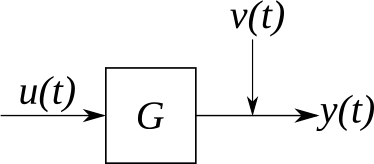
\includegraphics[width=.5\textwidth]{images/04system}
	\caption{Block diagram of system with input, output and noise signals.}
	\label{fig:04system}
\end{figure}

The expectation operator yields the average of the stochastic portion of the output. What we want to find is a linear operator that will give the average of the deterministic part as well. For that we use the extended expectation operator.
$$\bar{E}\{y(t)\} = \lim_{N\to\infty}\frac{1}{N}\sum_{t=1}^NE\{y(t)\}$$
When the expectation operator is used it takes the stochastic portion of the output and makes it deterministic, giving just a scalar value. The extended expectation operator averages the output, $y(t)$, over time to give a scalar as well.

The time-shifted input, $w(t)=G_0(q)u(t)$, is deterministic with
$$\bar{E}\{w(t)\} = \lim_{N\to\infty}\frac{1}{N}\sum_{t=1}^NE\{w(t)\}$$
and we typically assume $\bar{E}\{w(t)\}=0$.

\begin{example}
Given a deterministic signal, $u(t)$, as shown in Figure \ref{fig:04inputSignal} we can say that
$$lim_{N\to\infty}\frac{1}{N}\sum_{t=1}^NE\{u(t)\} = 0$$
This is shown as a block diagram in Figure \ref{fig:04detSignal} and makes it clear that $\lim_{N\to\infty}\frac{1}{N}\sum_{t=1}^Nw(t)=0$ since $u(t)=0$ and the system is linear.
\end{example}
$\lozenge$
\begin{figure}[ht!]
	\centering
	\includegraphics[width=.5\textwidth]{images/04inputSignal}
	\caption{Example of an input signal that tends to have zero-mean over long enough time periods.}
	\label{fig:04inputSignal}
\end{figure}

\begin{figure}[ht!]
	\centering
	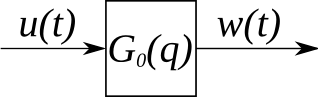
\includegraphics[width=.5\textwidth]{images/04detSignal}
	\caption{Block diagram of system with deterministic, zero-mean input signal.}
	\label{fig:04detSignal}
\end{figure}

\begin{definition}{Extended Expectation Operator}
$$\bar{E}\{y(t)\}=\lim_{N\to\infty}\frac{1}{N}\sum_{t=1}^NE\{y(t)\}$$
Typically, we assume that $E\{y(t)\}=0$ if $\bar{E}\{u(t)\}=0$ and $G_0(q)$ is BIBO stable. If the system is not BIBO stable then we get Brownian motion resulting in random walk.
\end{definition}

\begin{definition}{Quasi-stationary Signal}

Some process $u(t)$ is quasi-stationary if there exists some $c_1, c_2 \in\mathbb{R}$ such that
\begin{itemize}
\item $\bar{E}\{u(t)\} < c_1, ~\forall t$
\item $\bar{E}\{u(t)u(t-\tau)\} = R_u(\tau) < c_2, ~\forall \tau$
\end{itemize}
The first inequality means that the mean of the process must be bounded. The second inequality means that $u(t)$ correlated with itself and time-shifted a small amount should also be bounded and is known as the ``auto-covariance'' function.
\end{definition}

\begin{definition}{Covariance and Spectral Functions}

These are formal definitions and cannot actually be computed because they require an infinite number of samples. Later we will learn how to estimate their values.
\begin{itemize}
\item Auto-covariance function

$R_y(\tau) \triangleq \bar{E}\{y(t)y(t-\tau)\}, |\tau|\in\mathbb{N}$
\item Cross-covariance function

$R_{yu}(\tau) \triangleq \bar{E}\{y(t)u(t-\tau)\}, |\tau|\in\mathbb{N}$
\item Auto-spectral density function

$\phi_u(\w) \triangleq \sum_{\tau=-\infty}^\infty R_y(\tau)e^{-j\w\tau}$

This is the discrete-time Fourier transform (DTFT) of the auto-covariance function.
\item Cross-spectral density function

$\phi_{yu}(\w) \triangleq \sum_{\tau=-\infty}^\infty R_yu(\tau)e^{-j\w\tau}$

This is the DTFT of the cross-covariance function.
\end{itemize}
Note that $\w\in\mathbb{R}$ and $|\tau|\in\mathbb{N}$. To get from the spectral density functions to the covariance functions use the inverse Fourier transform: $R_y(\tau) = \frac{1}{2\pi}\int_{\w=-\pi}^\pi R_y(\tau)e^{j\w\tau}d\w$.
\end{definition}

\section{White Noise}
White noise, $e(t)$, is a zero-mean signal and is satisfied by the following properties:
\begin{itemize}
\item $\bar{E}\{e(t)\}=0$
\item $\bar{E}\{e(t)e(t-\tau)\} = R_e(\tau) = \begin{cases} \lambda>0, & \tau=0 \\ 0, & |\tau|\neq 0 \end{cases}$

The case when $\tau=0$ is known as the variance of the signal.
\item $\phi_e(\w) = \sum_{\tau=-\infty}^\infty \lambda\delta_d(t)e^{-j\w t} = \lambda e^{-j\w 0} = \lambda$

We only need to evaluate the $\delta$-function at time $t=0$. See Figure \ref{fig:04deltaFn}.
\item $\bar{E}\{e^2(t)\} = R_e(0) = \lambda = \frac{1}{2\pi}\int_{\w=-\pi}^\pi\phi_u(\w)e^{j\w\tau}d\w = \frac{1}{2\pi} \int_{\w=-\pi}^\pi\phi_u(\w)d\w$

where the exponential goes to one because $\tau=0$. This can be thought of as the surface under the auto-spectral density function between $[-\pi,\pi]$ and is equal to the variance of the signal.
\end{itemize}
\begin{figure}[ht!]
	\centering
	\includegraphics[width=.5\textwidth]{images/04deltaFn}
	\caption{A delta function at $t=0$ with magnitude of $\lambda$.}
	\label{fig:04deltaFn}
\end{figure}

\section{Uncorrelated Signals}
Consider two signals $u(t)$ and $v(t)$ that are not necessarily input and output. We say that $u\perp y$ or ``u is uncorrelated with y'' if $R_{yu}(\tau)=0 ~\forall \tau$.

\subsection{Application}
Consider the system $y(t)=G_0(q)u(t)+v(t)$. The cross-correlation function is found as
\begin{align*}
\bar{E}\{y(t)u(t-\tau)\} &= \bar{E}\{G_0(q)u(t)u(t-\tau)\} + \bar{E}\{v(t)u(t-\tau)\} \\
&= \bar{E}\{G_0(q)u(t)u(t-\tau)\} \\
&\Rightarrow R_{yu}(\tau) = G_0(q)R_u(\tau)
\end{align*}
The term $\bar{E}\{v(t)u(t-\tau)\} = 0$ based on the assumption that since $u(t)$ is a designed and deterministic signal then it is highly unlikely that the input and the noise are correlated.

\section{Effects of Dynamics/Filtering}
\subsection{Cross-covariance Function}
Let $\{u(t)\}$ be white noise, $y(t)=G_0(q)u(t)+v(t)$, $u\perp v$ and $G_0(q)=\sum_{k=0}^\infty g(k)q^{-k}$. Note that $\{u(t)\}$ is white but known. How do we find $R_{yu}(\tau)$?

Start with
\begin{align*}
R_{yu}(\tau) &= G_0(q)R_u(\tau) \\
R_u(\tau) &= \begin{cases} \lambda, & \tau=0 \\ 0, & \tau\neq 0 \end{cases} = \lambda\delta_d(\tau)
\end{align*}
Substituting the second equation into the first is equivalent to getting the impulse response of the system as described by the coefficients $g(k)$ so that
$$R_{yu}(\tau) = \lambda g(\tau)$$

\begin{example}
Let $G_0(q)$ be a mass-spring-damper system with low amounts of damping. Given an impulse as input the output signal will oscillate at some frequency while dying down due to the damping. See Figure \ref{fig:04dimSine}.
\end{example}
$\lozenge$
\begin{figure}[ht!]
	\centering
	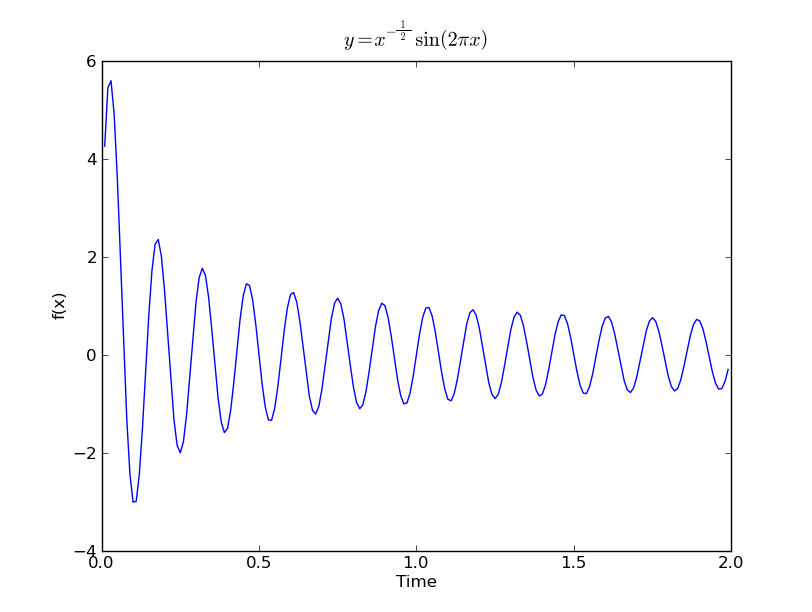
\includegraphics[width=.5\textwidth]{images/04dimSine}
	\caption{A diminishing sine wave representing the impulse response in a mass-spring-damper system with low amounts of damping.}
	\label{fig:04dimSine}
\end{figure}

\subsection{Auto-spectral Density Function}
\begin{example}
Let $\{e(t)\}$ be white noise where $E\{e(t)\}=0$, $v(t)=H_0(q)e(t)$. How do we find $\phi_v(\w)$?
\begin{align*}
\phi_v(\w) &= \mathcal{F}\{R_v(\tau)\} \\
&= \mathcal{F}\{E\{v(t)v(t-\tau)\}\} \\
&= \mathcal{F}\{E\{H_0(q)e(t)H_0(q)e(t-\tau)\}\} \\
&= \vectornorm{H_0(e^{j\w})}^2\phi_e(\w) \\
&= \vectornorm{H_0(e^{j\w}}^2\cdot\lambda
\end{align*}
The final equality uses the fact that $\phi_e(\w)=\lambda$ because the noise is white. This shows that applying the filter $H_0(q)$ changes the shape of the input of white noise. After the filter the white noise contains much lower frequencies so the noise, $v(t)$, is colored. See Figure \ref{fig:04filteredNoise}.
\end{example}
$\lozenge$
\begin{figure}[ht!]
	\centering
	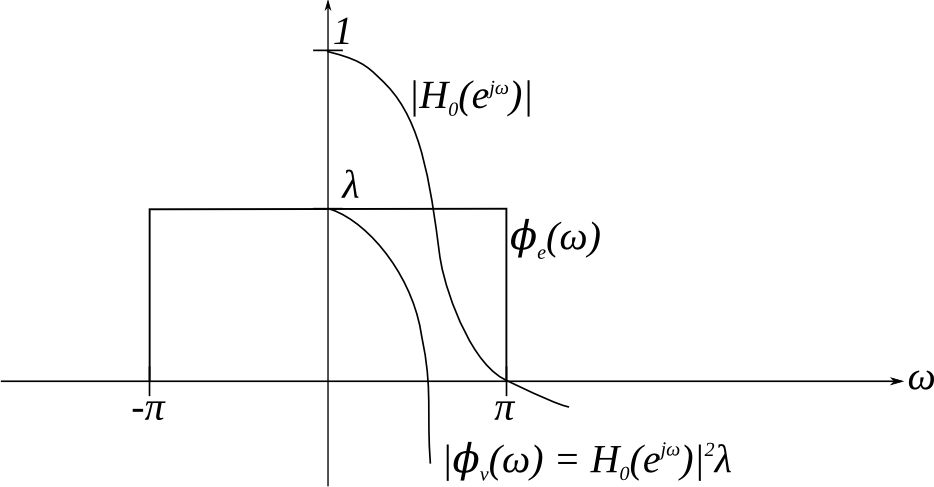
\includegraphics[width=.7\textwidth]{images/04filteredNoise}
	\caption{Effect of filtering white noise.}
	\label{fig:04filteredNoise}
\end{figure}

\subsection{Cross-spectral Density Function}
\begin{example}
How do we find $\phi_{yu}(\w)$?
$$\phi_{yu}(\w) = \mathcal{F}\{R_{yu}(\tau)\} = \lambda G_0(e^{j\w})$$
The Fourier transform of an implulse response yields the transfer function. This allows us to back out the Markov parameters.
\end{example}
$\lozenge$

\begin{example}
Given $y(t)=w(t)+v(t)$ we get
\begin{align*}
\phi_y(\w) &= \lambda\vectornorm{G_0(e^{j\w}}^2 + \phi_v(\w) \\
\phi_v(\w) &= \phi_y(\w) - \vectornorm{\phi_{yu}(\w)}
\end{align*}
$\phi_v(\w)$ is the noise that was acting on the system and can now be identified.
\end{example}
$\lozenge$

\section{Effect of Periodogram}
This is covered in Ljung, pages 31-33.
\begin{definition}{Periodogram}

Essentially, the periodogram $\hat{\phi}_y(\w)$ is a cheap way of estimating the spectrum, or the frequency contents, of a signal.
\begin{align*}
\phi_y(\w) &= \mathcal{F}\{R_u(\tau)\} \\
\hat{\phi}_y(\w) &= y(\w)y^*(\w) \\
y(\w) &= \sum_{t=1}^Ny(t)e^{-j\w t}, |t|\in\mathbb{N} \\
\hat{\phi}_y(\w) &= |y(\w)|^2 = y(\w)y^*(\w)
\end{align*}
Recall that the Fourier transform of the convolution operator is the multiplication operator.
\end{definition}

\begin{theorem}
This is Theorem 2.1 from Ljung on page 31.
If the output is noise-free such that $y(t)=G_0(q)u(t)$ then
\begin{align*}
Y_N(\w) &= \frac{1}{\sqrt{N}}\sum_{t=1}^Ny(t)e^{-j\w t} \\
U_N(\w) &= \frac{1}{\sqrt{N}}\sum_{t=1}^Nu(t)e^{-j\w t} \\
Y_N(\w) &= G_0(e^{j\w})U_N(\w) + R_N(\w)
\end{align*}
The first two equalities are discrete Fourier transforms. $Y_N(\w)$ and $U_N(\w)$ are finite F.T.s and $R_N(\w)$ is an infinite Fourier transform. This leads to
$$|R_N(\w)| \leq 2\cdot C_w\cdot \frac{C_g}{\sqrt{N}}$$
where $|u(t)|<C_w ~\forall t$, $C_g=\sum_{k=0}^\infty k|g_k|<\infty$ if the system is BIBO stable.
\end{theorem}
Note that $R_N(\w)$ is the noise due to the inital and end conditions that can be bounded. This noise arises because when we use the F.T. we automatically make the assumption that the signal is periodic even when they are not periodic as discussed in Lecture 2.


\end{document}

%%%%%%%%%%%%%%%%%%%%%%%%%%%%%%%%%%%%%%%%%%%%%%%%%%%%%%%%%%%%%